\subsubsection{Deletion Latency}
We now estimate the impact of rule deletions.
We use bursts of operations as before.
Denote
$T(r_i)$ as the first time we stopped observing packets matching rule $r_i$
from the intended port of the rule action. We define deletion latency
as $T(r_i)-T(r_{i-1})$.

\begin{figure}[!tb]
\centering
\subfloat[100 rules in table \label{fig:bcm_del_same_burst_100}]
  {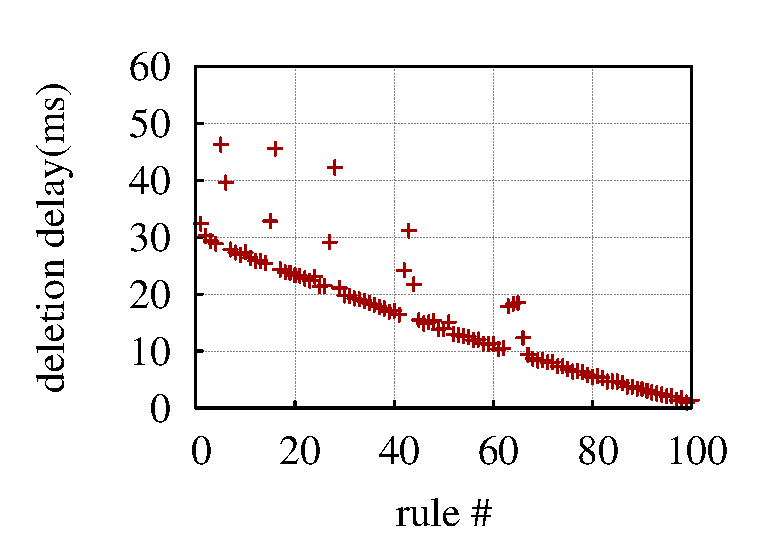
\includegraphics[width=.50\linewidth]{./figs/jan27_bcm_del_same_burst_100.eps}}\hfill
%\subfloat[burst size 100, increasing priority.\label{fig:bcm_del_incr_burst_100}]
%  {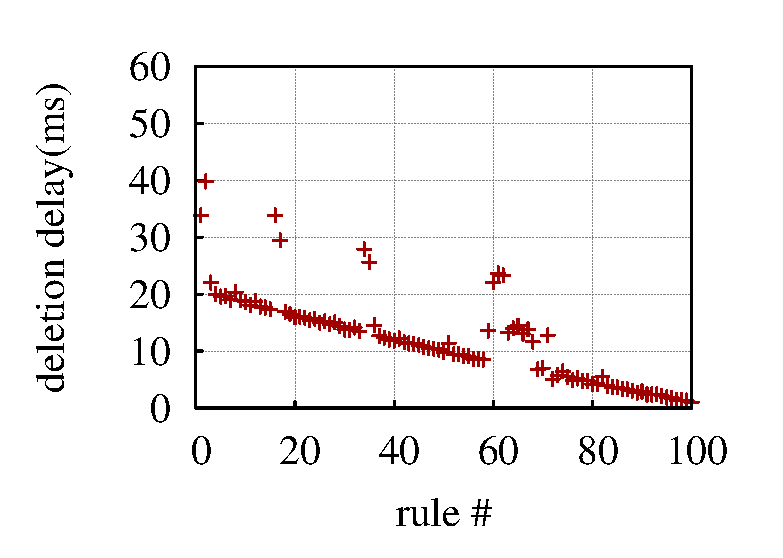
\includegraphics[width=.30\linewidth]{./figs/jan27_bcm_del_incr_burst_100.eps}}\hfill
\subfloat[200 rules in table \label{fig:bcm_del_same_burst_200}]
  {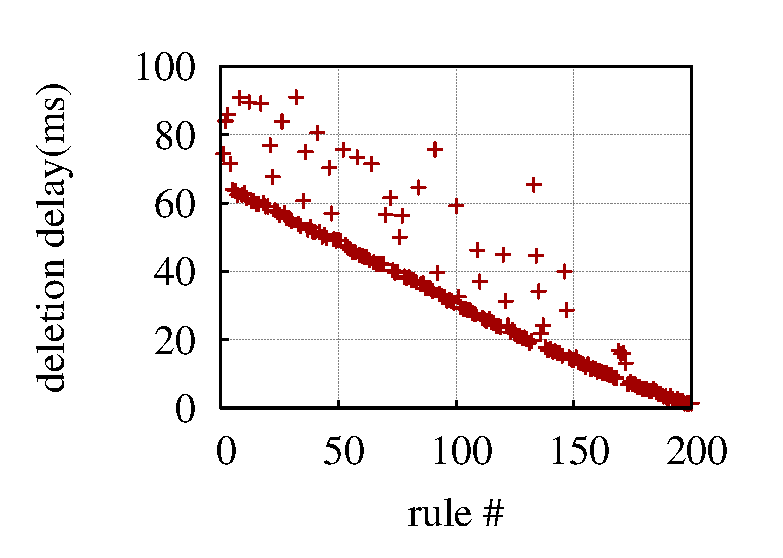
\includegraphics[width=.50\linewidth] {./figs/jan27_bcm_del_same_burst_200.eps}}
\compactcaption{ {\bf \BroadcomOne} per-rule {\bf del.} latency, same priority}
\label{fig:occupancy-broadcom-deletion}
\end{figure}

\begin{figure}[!tb]
\centering
\subfloat[100 rules in table\label{fig:intel_del_same_burst_100}]
  {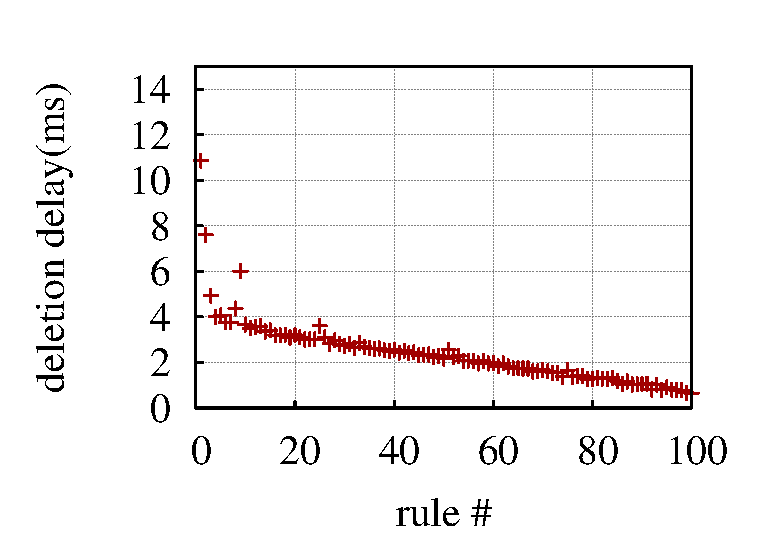
\includegraphics[width=.50\linewidth]{./figs/jan27_intel_del_same_burst_100.eps}}\hfill
%\subfloat[burst size 100, increasing priority.\label{fig:intel_del_incr_burst_100}]
%  {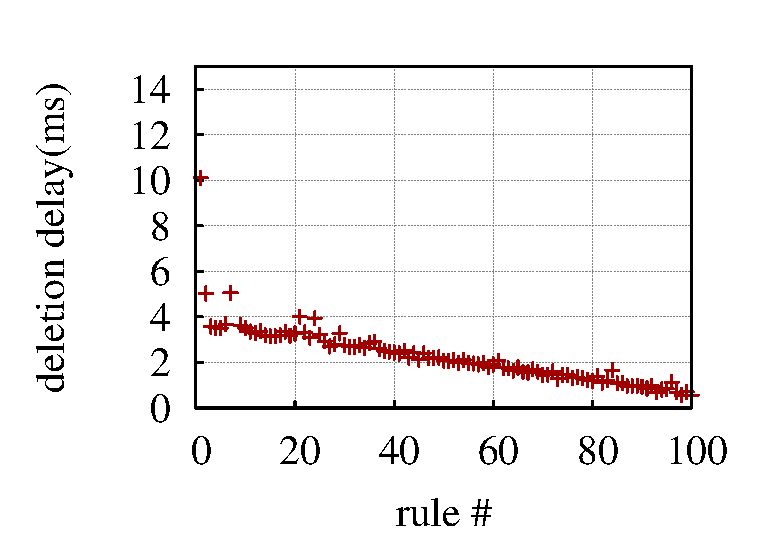
\includegraphics[width=.30\linewidth]{./figs/jan27_intel_del_incr_burst_100.eps}}\hfill
\subfloat[200 rules in table \label{fig:intel_del_same_burst_200}]
  {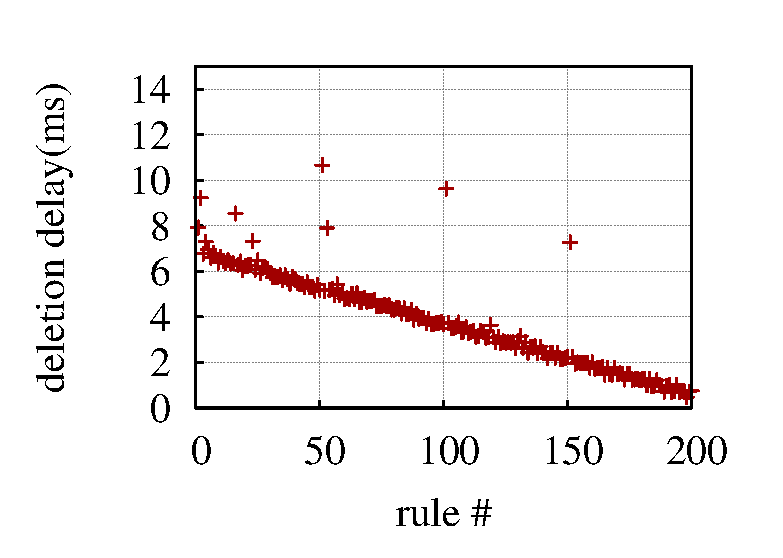
\includegraphics[width=.50\linewidth]{./figs/jan27_intel_same_burst_200.eps}}
\compactcaption{{\bf \Intel} per-rule {\bf del.} latency, same priority}
\label{fig:occupancy-intel-deletion}
\end{figure}

\minisection{Table Occupancy} We pre-insert $S$ rules into a switch, all with
the same priority. We then delete one rule at a time, sending deletion
requests back-to-back. The results for \BroadcomOne at $S=100$ and $S=200$
are shown in \figsref{fig:bcm_del_same_burst_100}{fig:bcm_del_same_burst_200},
respectively. We see that per rule deletion delay decreases as the table occupancy drops. We see a similar trend for Intel (\figsref{fig:intel_del_same_burst_100}{fig:intel_del_same_burst_200}) \BroadcomThree and \IBM (figure not shown).

%  and
% ~\ref{fig:occupancy-intel-deletion}, the per rule deletion delay
% decreases as the table occupancy drops.


\begin{figure}[!tb]
\centering
% \subfloat[burst size 100, same priority.\label{fig:bcm_del_same_burst_100}]
%   {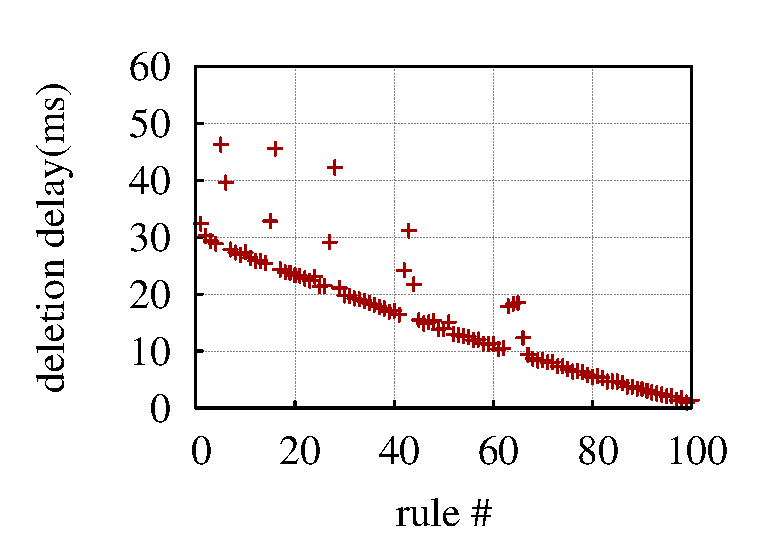
\includegraphics[width=.30\linewidth]{./figs/jan27_bcm_del_same_burst_100.eps}}\hfill
\subfloat[increasing priority\label{fig:bcm_del_incr_burst_100}]
  {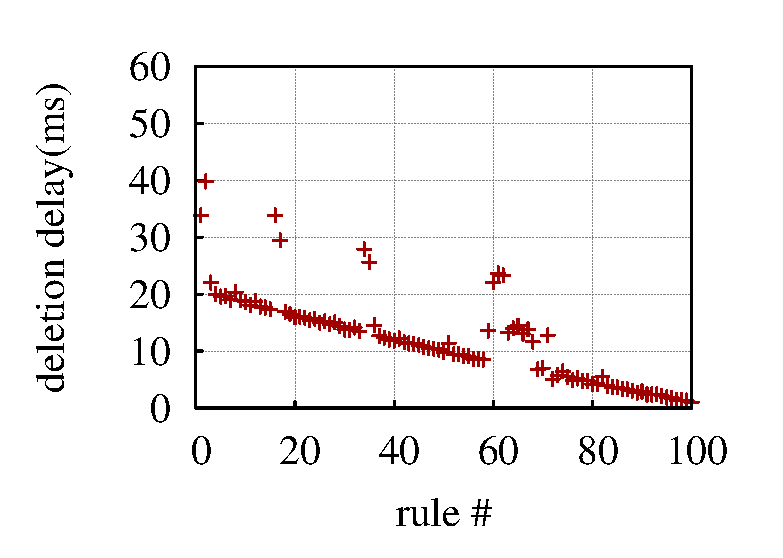
\includegraphics[width=.50\linewidth]{./figs/jan27_bcm_del_incr_burst_100.eps}}\hfill
\subfloat[decreasing priority\label{fig:bcm_del_decr_burst_100}]
  {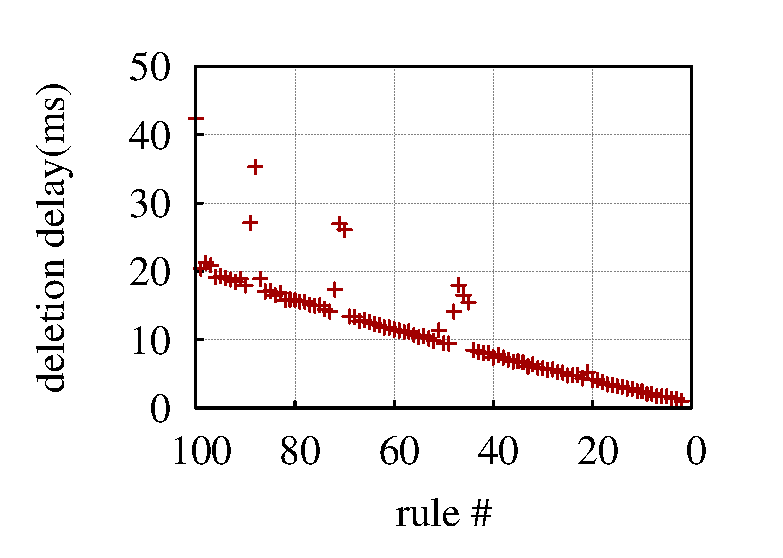
\includegraphics[width=.50\linewidth]{./figs/jan27_bcm_del_decr_burst_100.eps}}
\compactcaption{{\bf \BroadcomOne} priority per-rule {\bf del.} latency, 
    B=100}
\label{fig:priority-broadcom-deletion}
\end{figure}

\begin{figure}[!tb]
\centering
%\subfloat[burst size 100, same priority.\label{fig:jan27_intel_del_same_burst_100}]
%  {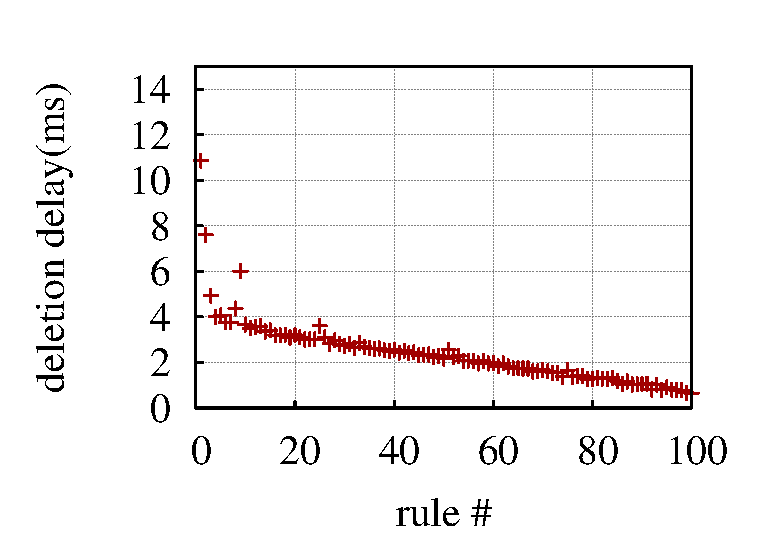
\includegraphics[width=.24\linewidth]{./figs/jan27_intel_del_same_burst_100.eps}}\hfill
%\subfloat[burst size 100, increasing priority.\label{fig:jan27_intel_del_incr_burst_100}]
%  {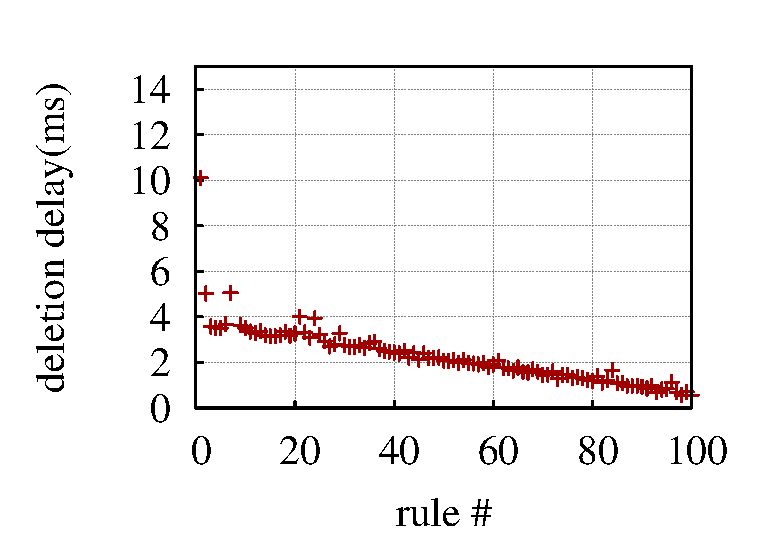
\includegraphics[width=.24\linewidth]{./figs/jan27_intel_del_incr_burst_100.eps}}\hfill
%\subfloat[burst size 100, decreasing priority.\label{fig:jan27_intel_del_decr_burst_100}]
%  {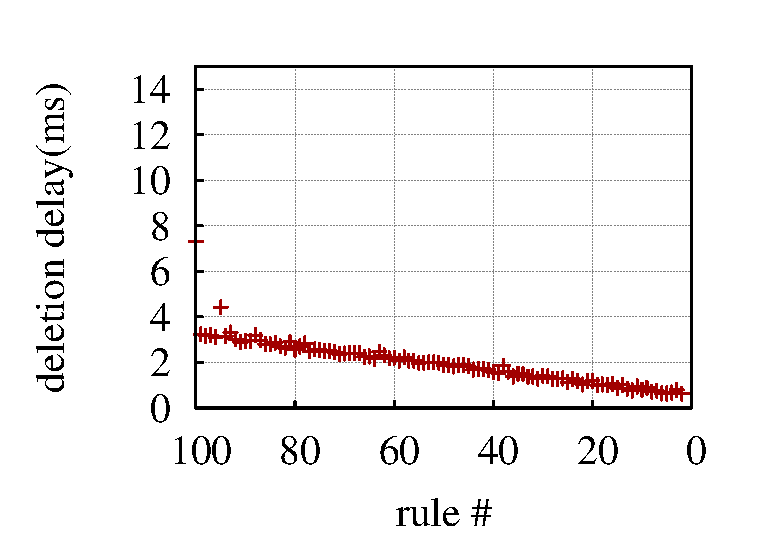
\includegraphics[width=.24\linewidth]{./figs/jan27_intel_del_decr_burst_100.eps}

% \subfloat[burst size 100, same priority.\label{fig:intel_intel_del_same_burst_100}]
%   {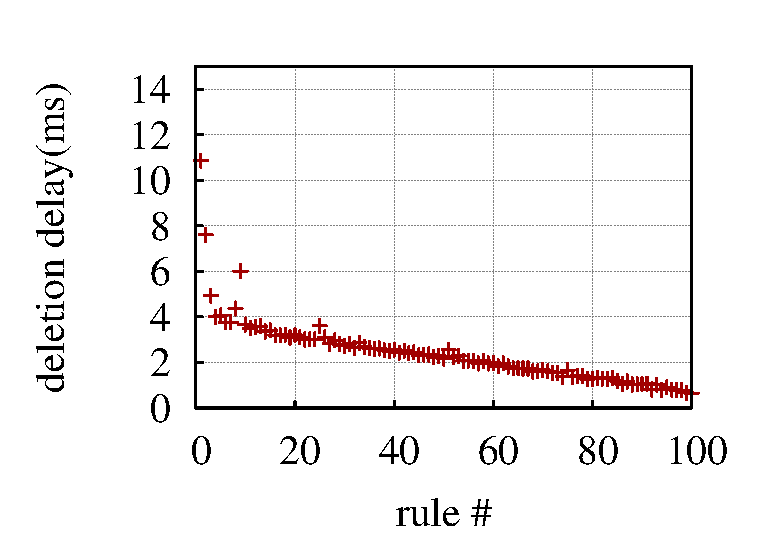
\includegraphics[width=.30\linewidth]{./figs/jan27_intel_del_same_burst_100.eps}}\hfill
\subfloat[increasing priority\label{fig:intel_del_incr_burst_100}]
  {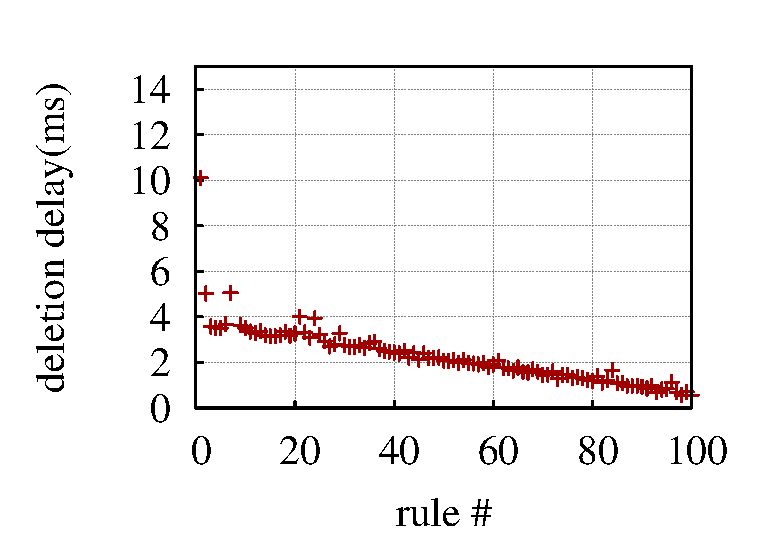
\includegraphics[width=.50\linewidth]{./figs/jan27_intel_del_incr_burst_100.eps}}\hfill
\subfloat[decreasing priority\label{fig:intel_del_decr_burst_100}]
  {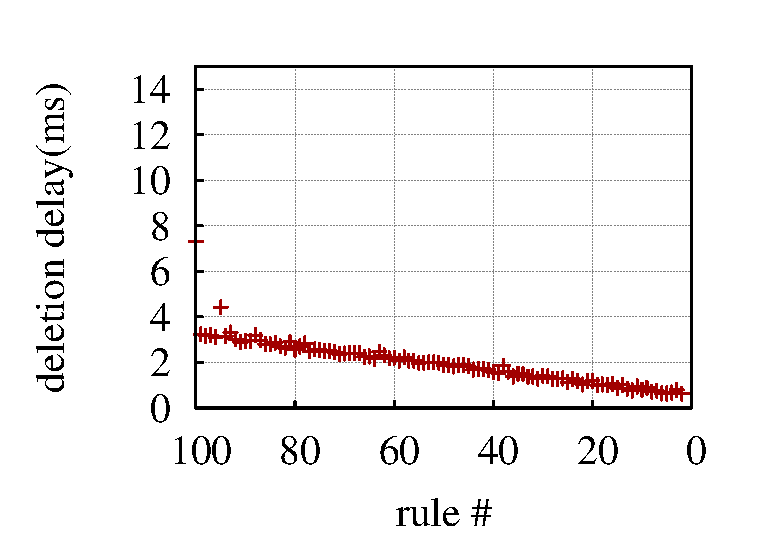
\includegraphics[width=.50\linewidth]{./figs/jan27_intel_del_decr_burst_100.eps}}

\compactcaption{{\bf Intel} priority per-rule {\bf del.} latency, B=100}
\label{fig:priority-intel-deletion}
\end{figure}


\minisection{Rule Priorities} We start with $B$ existing rules in the switch, 
and delete one rule at a time
%,``with'' and ``without priority''. In the former case, 
%we delete rules 
in increasing and decreasing priority order. 
For \BroadcomOne (\figref{fig:priority-broadcom-deletion}), \BroadcomThree
(figure not shown) Intel (\figref{fig:priority-intel-deletion}) and \IBM, deletion 
is not affected by the priorities of rules in the table or the order of
deletion. %\aaron{Where are the without priority results?}


\minisection{\bf Root cause} Since deletion delay decreases with rule number 
in all cases, we conclude that deletion is incurring TCAM reordering.
% We observe that rule priority pattern does not affect deletion delay for both
% Broadcom and Intel. However, flow table occupancy affects deletion delay
% significant. Deletion delay can be much higher than insertion delay with same
% priority. 
% This seems to indicate that deletion incurs TCAM reordering in all
% cases in both switch architectures.
We also observe that processing rule timeouts at the switch does not
noticeably impact \flowmod operations. Given these two observations, we
recommend allowing rules to time out rather than explicitly deleting them, if
possible.

% LocalWords:  pre Broadcom TODO butbound TCAM
